\documentclass{article}
\usepackage{amsmath}
\usepackage{amssymb}
\newcommand*{\qed}{\hfill\ensuremath{\blacksquare}}
\usepackage{graphicx}
\graphicspath{{.}}

\title{Computational Linear Algebra, Module 9}
\author{Maya Shende}
\date{Due: April 11th, 2018}

\begin{document}
\maketitle

\begin{enumerate}

%exercise 1
\item Yes, this does draw the function $g(x) = x-\frac{5}{3}x^3$

%exercise 2
\item When more terms are added to the approximation function, we see that it looks like the sine function

%exercise 3
\item 
Errors for interval $[0, 2\pi]:$\\
\begin{tabular}{|c|c|}
	\hline
	n=3	&44.03945\\
	n=5 	&38.71829\\
	n=7	&18.99292\\
	n=13	&0.22859\\	
	\hline
\end{tabular}\\
The difference between $n=3$ and $n=13$ is $44.03945-0.22859 = 43.81086$. The errors for $n=3$ and $n=13$ for the interval $[0,\pi]$ are: $n=3 \rightarrow 1.13981$ and $n=13 \rightarrow 4.30594 \times 10^{-6}$\\

For the interval $[0, \pi/2]$, the errors are $n=3 \rightarrow 0.01836$ and $n=13 \rightarrow 4.30594 \times 10^{-11}$\\

The error at each point is multiplied by deltaX because we are calculating the area between the two curves to find the error. 

%exercise 4
\item Taylor series expansion: $\sin{x} = x - \frac{x^3}{3!} + \frac{x^5}{5!} - \frac{x^7}{7!} + \frac{x^9}{9!} - \dots$. The coefficients printed in the alpha array are the same as those we saw in the earlier exercise. 

%exercise 5
\item $k=3:$ \\
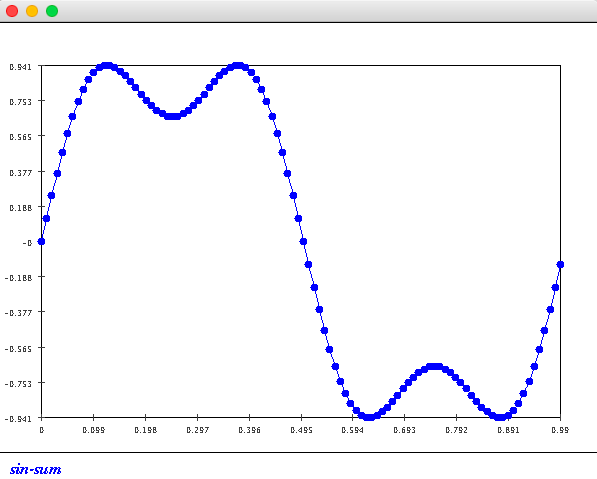
\includegraphics[scale=0.3]{exercise5_k3}\\
$k=5:$ \\
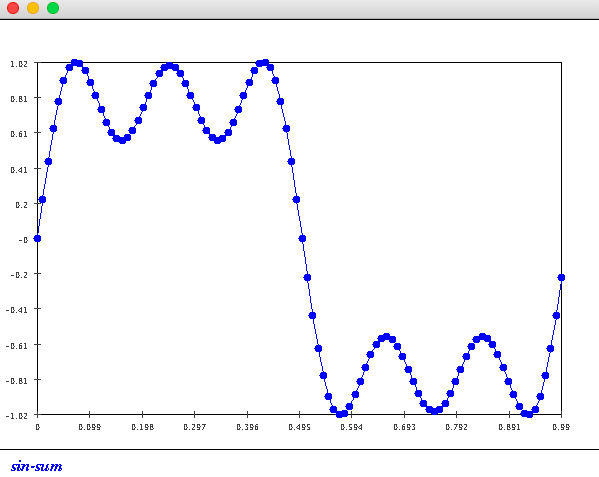
\includegraphics[scale=0.3]{exercise5_k5}\\
$k=7:$ \\
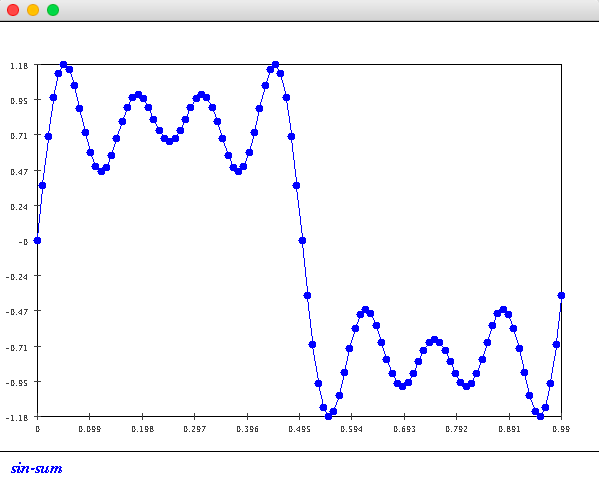
\includegraphics[scale=0.3]{exercise5_k7}\\
$k=9:$ \\
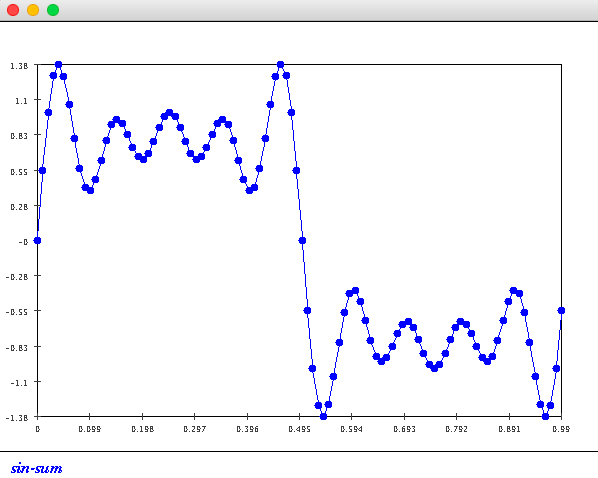
\includegraphics[scale=0.3]{exercise5_k9}\\
$k=11:$ \\
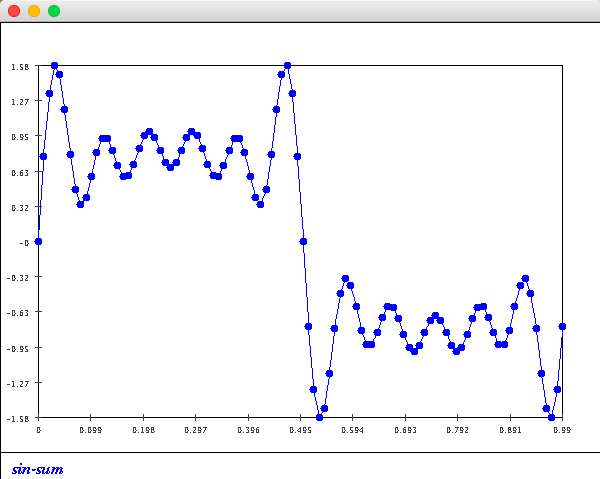
\includegraphics[scale=0.3]{exercise5_k11}

%exercise 6
\item No linear combination of $\sin{(2\pi kx)}$ can approximate any step function. For example, $h(x) = $

\[
\begin{cases} 
      1 & x< 0 \\
      3 & 0\leq x\leq 20 \\
      5 & 20< x 
\end{cases}
\]

%exercise 7
\item The second graph that is output by this program is a subsection of the first graph, and this is a fractal so the subsection looks like the full graph.

%exercise 8
\item $k=0 \rightarrow$ evaluates to 1\\
$k=1 \rightarrow$ evaluates to $n$\\
$k=n-1 \rightarrow$ evaluates to $n$, which is the same as when $k=1$\\
$k=n \rightarrow$ evaluates to 1, which is the same as when $k=0$

%exercise 9
\item ${n\choose k} = \frac{n!}{k! (n-k)!} \rightarrow$ this is derived by taking the total number of combinations possible, and dividing out the repeated combinations.\\
\begin{tabular}{|c|c|}
	\hline
	k	& ${n\choose k}$\\
	\hline
	0	& 1\\
	\hline
	1	& 5\\
	\hline
	2	& 10\\
	\hline
	3	& 10\\
	\hline
	4	& 5\\
	\hline
	5	& 1\\
	\hline
\end{tabular}

%exercise 10
\item We know that ${n\choose k} = \frac{n!}{k!(n-k)!}$, ${n-1\choose k} = \frac{(n-1)!}{k!(n-1-k)!}$ and ${n-1\choose k-1} = \frac{(n-1)!}{(k-1)!(n-k)!}$. So now we have:
\begin{eqnarray*}
	{n-1\choose k} + {n-1\choose k-1} &=& \frac{(n-1)!}{k!(n-1-k)!} + \frac{(n-1)!}{(k-1)!(n-k)!}\\
	&=& \frac{(n-1)!(n-k) + k(n-1)!}{k!(n-k)!}\\
	&=& \frac{n! - k(n-1)! + k(n-1)!}{k!(n-k)!}\\
	&=& \frac{n!}{k!(n-k)!}\\
	&=& {n\choose k} 
\end{eqnarray*} 
Therefore, ${n\choose k} = {n-1\choose k} + {n-1\choose k-1}$ \qed

$n\choose k$ is a symmetric function because of how choosing combinations works. Pascal's Triangle:\\
\begin{tabular}{ccccccccc}
	\hfill	&\hfill	&\hfill	& \hfill 	& 1	&\hfill	&\hfill	&\hfill	&\hfill\\
	\hfill	&\hfill	&\hfill	&1	& \hfill	& 1	& \hfill	&\hfill	&\hfill\\
	\hfill	&\hfill	&1	&\hfill	&2	&\hfill	&1	&\hfill	&\hfill\\
	\hfill	&1	&\hfill	&3	&\hfill	&3	&\hfill	&1	&\hfill\\
	1	&\hfill	&4	&\hfill	&6	&\hfill	&4	&\hfill	&1
\end{tabular}

Each row of Pascal's Triangle gives the values of $n\choose k$, where k is the column of the row and n is the row number. 

%exercise 11
\item 
\begin{tabular}{|c|c|c|}
	\hline
	n	&numCalls	&numCallsRecursive \\
	\hline
	5	&62	&58 \\
	\hline
	10	&222		&2037 \\
	\hline
	20	&842		&2097131\\
	\hline
\end{tabular}

For large enough n, the recursive definition is no longer efficient. 

%exercise 12
\item 
\begin{eqnarray*}
	RHS &=& \frac{n}{k}{{n-1}\choose{k-1}}\\
	&=& \frac{n}{k}\left(\frac{(n-1)!}{(k-1)!(n-1-(k-1))!}\right)\\
	&=& \frac{n}{k}\left(\frac{(n-1)!}{(k-1)!(n-k)!}\right)\\
	&=& \frac{n!}{k!(n-k)!}\\
	&=& {{n}\choose{k}}
\end{eqnarray*}
\qed\\
\begin{tabular}{|c|c|c|}
	\hline
	n	&numCalls	&numCallsRecursive \\
	\hline
	5	&62	&58 \\
	\hline
	10	&222		&2037 \\
	\hline
	20	&842		&2097131\\
	\hline
\end{tabular}\\
The return type is double due to the $\frac{n}{k}$ that is in the formula in the iterative method.

%exercise 13
\item 
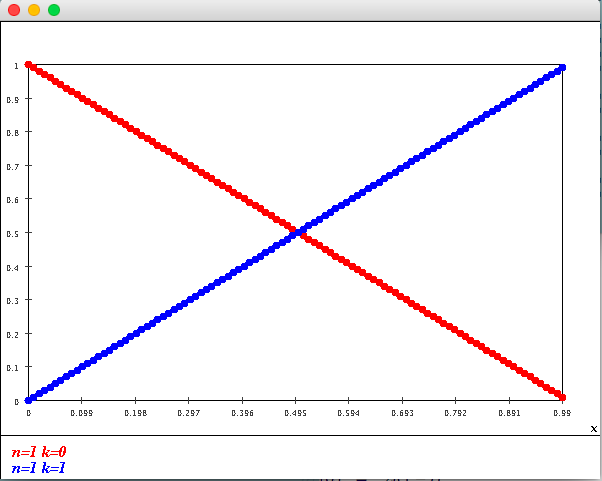
\includegraphics[scale=0.4]{bernstein_1}

%exercise 14
\item 
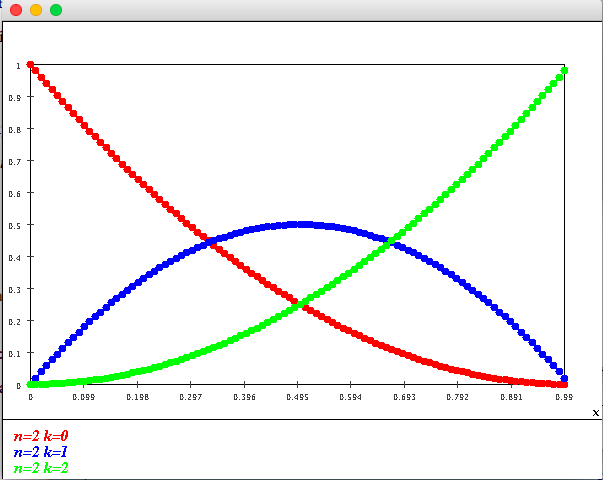
\includegraphics[scale=0.3]{bernstein_2}
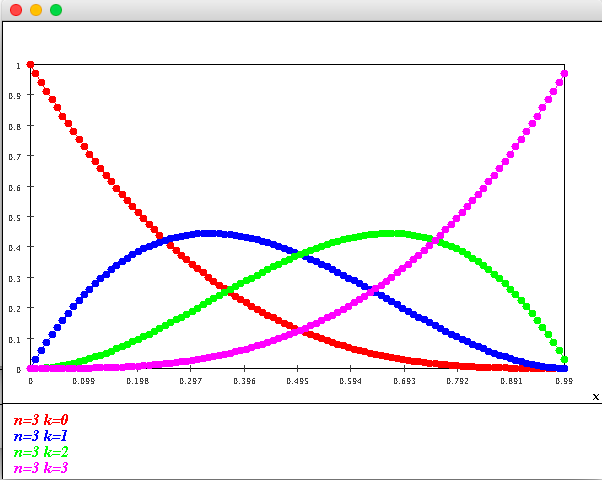
\includegraphics[scale=0.3]{bernstein_3}

%exercise 15
\item For $n=5$, there were 1800 numCalls and 5800 numRecursiveCalls.

%exercise 16
\item Since $a<b$, we have 
\begin{eqnarray*}
	(1-t)a + tb &>& (1-t)a + ta\\
	&=& a(1-t+t)\\
	&=& a
\end{eqnarray*}
and we have
\begin{eqnarray*}
	(1-t)a + tb &<& (1-t)b + tb\\
	&=& b(1-t+t)\\
	&=& b
\end{eqnarray*}
. So, $a < (1-t)a + tb < b$. Therefore, $(1-t)a + tb \in [a,b]$. 

%exercie 17
\item $B_1 = \left\{{{1}\choose{0}} (1-t), {{1}\choose{1}} (t)\right\}$\\
$B_2 = \left\{{{2}\choose{0}} (1-t)^2, {{2}\choose{1}} (t)(1-t), {{2}\choose{2}} t^2 \right\}$\\
$B_3 = \left\{{{3}\choose{0}} (1-t)^3, {{3}\choose{1}} (t)(1-t)^2, {{3}\choose{2}} t^2(1-t), {{3}\choose{3}} t^3 \right\}$\\

%exercise 18
\item Suppose $B_n^{'}$ is a basis. Then, \\
$p(t) = a_0(1-t)^n + a_1t(1-t)^{n-1} + \dots + a_nt^n$. \\
Now, we can say that $a_k = b_k {{n}\choose{k}}$ for $k\leq n$ since each of these combinations is a constant, and $b_k$ is a constant for $k \leq n$. So, we now have\\
$p(t) = b_0{{n}\choose{0}}(1-t)^n + b_1{{n}\choose{1}}t(1-t)^{n-1} + \dots + b_n{{n}\choose{n}}t^n$. \\
Therefore, $B_n$ is also a basis. \qed

%exercise 19
\item 
\begin{eqnarray*}
	RHS &=& t^k(1-t)^{n+1-k} + t^{k+1}(1-t)^{n-k}\\
	&=& t^k((1-t)^{n+1-k}+t(1-t)^{n-k})\\
	&=& t^k(1-t)^{n-k}(1-t+t)\\
	&=& t^k(1-t)^{n-k} 
\end{eqnarray*}
\qed

%exercise 20
\item We want to show that $p_1 = at + b = \alpha(1-t) + \beta(t)$. So, 
\begin{eqnarray*}
	at+b &=& \alpha - \alpha t + \beta t\\
	at+b &=& \alpha - (\alpha - \beta) t\\
	a &=& -\alpha + \beta\\
	b &=& \alpha
\end{eqnarray*}
Therefore, we have found integer coefficients such that $(1-t)$ and $t$ are a linear combination for any polynomial of degree 1. 

%exercise 21
\item added code:\\
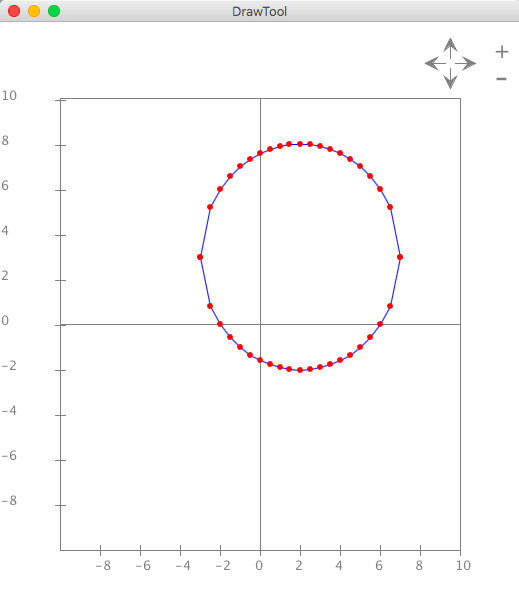
\includegraphics[scale=0.4]{exercise21} 

%exercise 22
\item You can complete the circle by saving the initial calculated x and y values, and then drawing the curve between the last calculated values and these first calculated values:\\
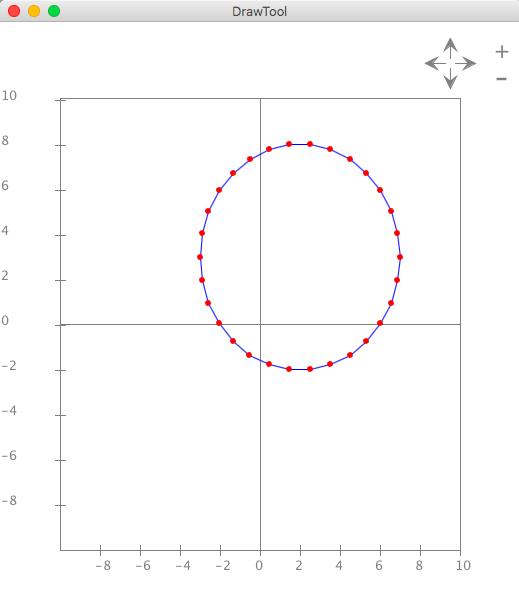
\includegraphics[scale=0.4]{exercise22}

%exercise 23
\item with rotation:\\
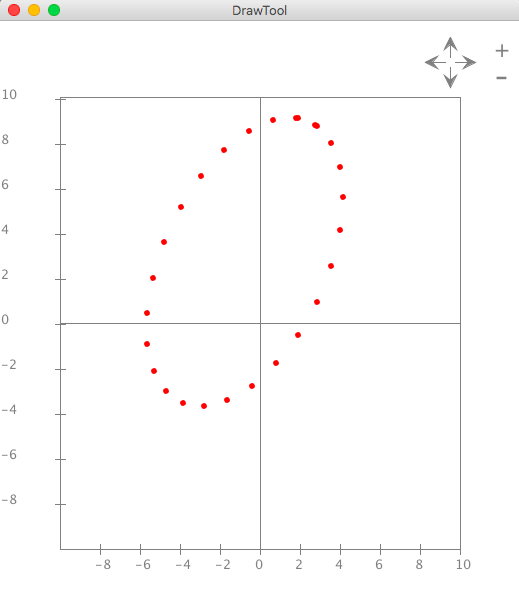
\includegraphics[scale=0.3]{exercise23_with_rotation}\\
without rotation:\\
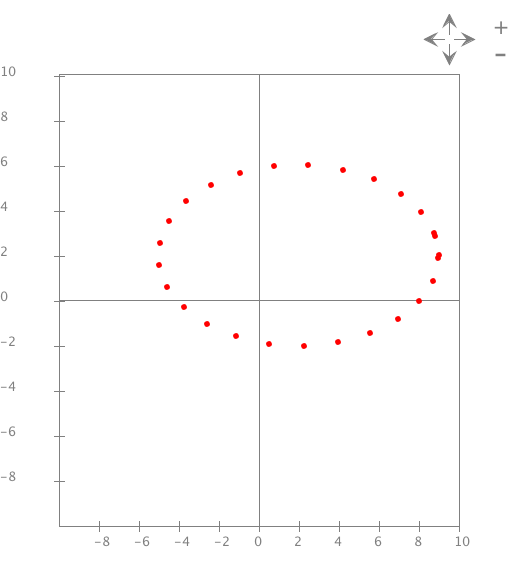
\includegraphics[scale=0.3]{exercise23_without_rotation}\\
with translation:\\
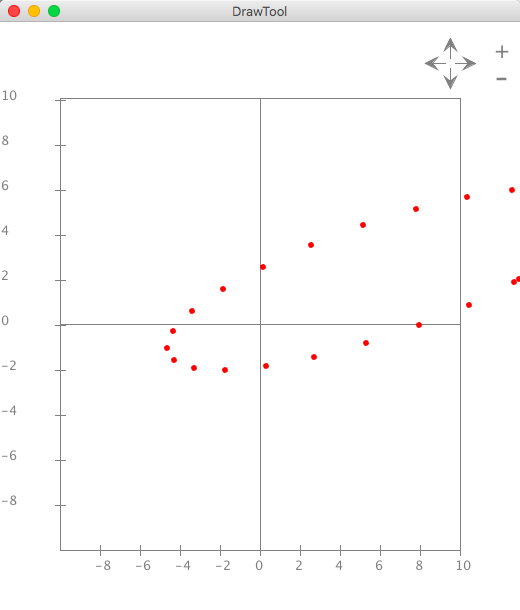
\includegraphics[scale=0.3]{exercise23_with_translation}

%exercise 24
\item Without transform:\\
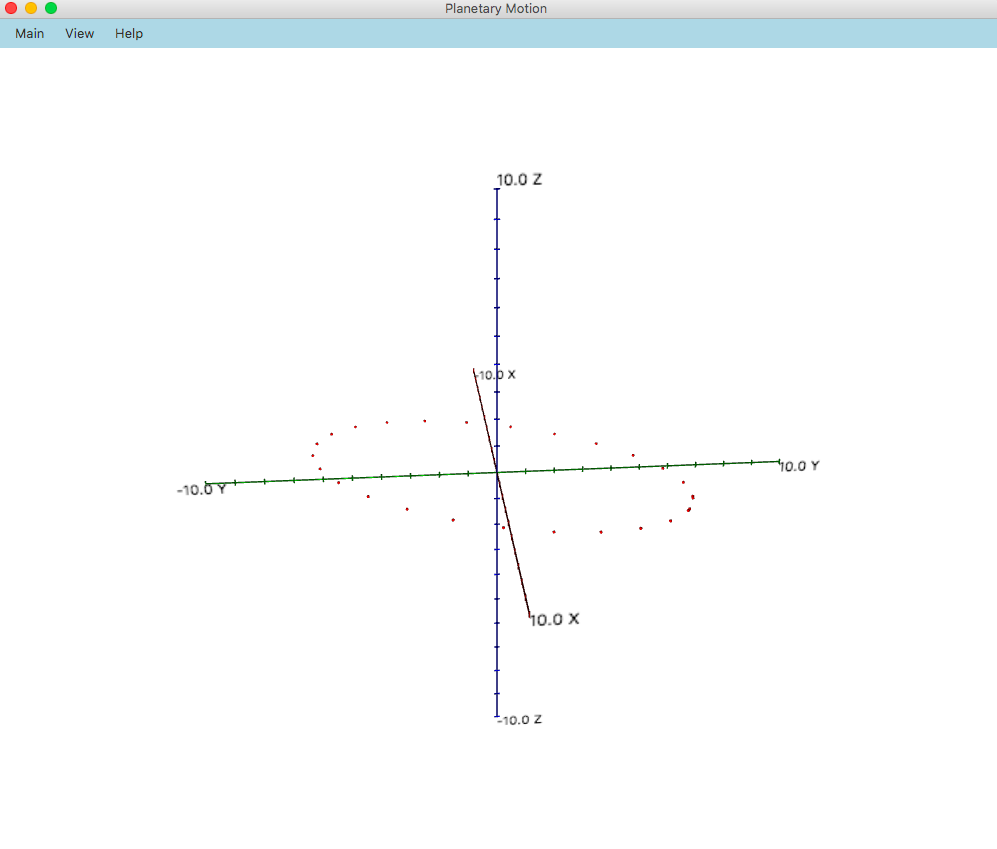
\includegraphics[scale=0.3]{exercise24_without_transform}\\
With transform:\\
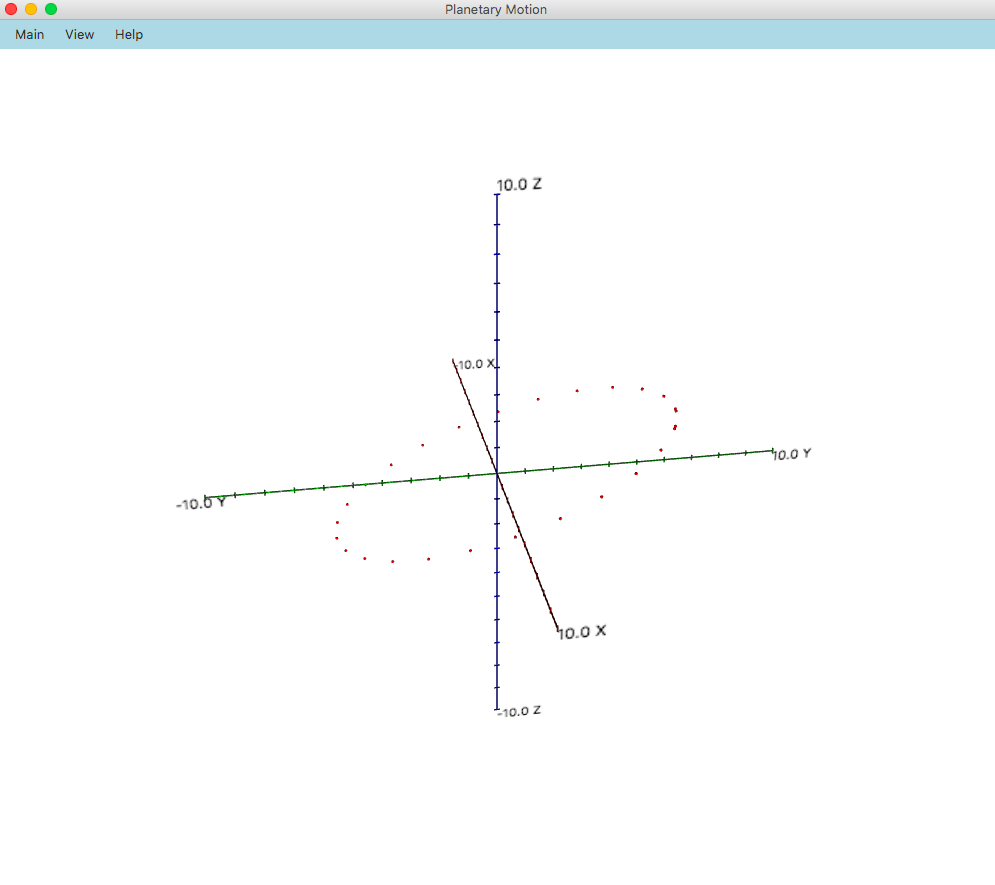
\includegraphics[scale=0.3]{exercise24_with_transform}

%exercise 25
\item 
\begin{enumerate}
	\item Since $x_0 < x_1$, 
	\begin{eqnarray*}
		tx_0 + (1-t)x_1 &>& tx_0 + (1-t)x_0\\
		&=& x_0(t+1-t)\\
		&=& x_0
	\end{eqnarray*}
	and 
	\begin{eqnarray*}
		tx_0 + (1-t)x_1 &<& tx_1 + (1-t)x_1\\
		&=& x_1(t+1-t)\\
		&=& x_1
	\end{eqnarray*}
The same argument can be made for when $x_1 < x_0$, $x_1 \leq x(t) \leq x_0$. 
	\item The slope between the endpoints $(2, 3)$ and $(5, 9)$ is 2. So, now if we plug this into the point-slope form, and use $x(t)$ and $y(t)$ as our $(x, y)$ point that we are looking at, we have:
	\begin{eqnarray*}
		y - 3 &=& 2(x-2)\\
		y(t) - 3 &=& 2(x(t) - 2)\\
		(3t + 9(1-t)) - 3 &=& 2((2t + 5(1-t))-2)\\
		6-6t &=& 2(3 - 3t)\\
		6 - 6t &=& 6-6t
	\end{eqnarray*}
	Therefore, each point $(x(t), y(t))$ is on the line segment between the end points. 
	\item The poitns fall on the same line as the line segment, but they do not fall on the actual line segment between the two endpoints. 
	\end{enumerate}

%exercise 26
\item image:\\
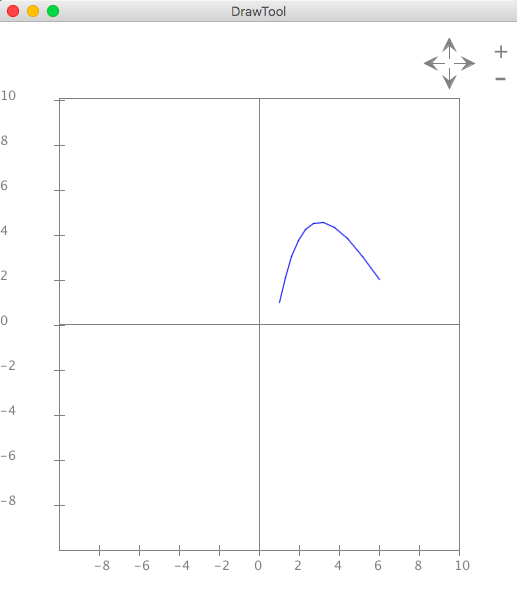
\includegraphics[scale=0.3]{exercise26}

%exercise 27
\item image:\\
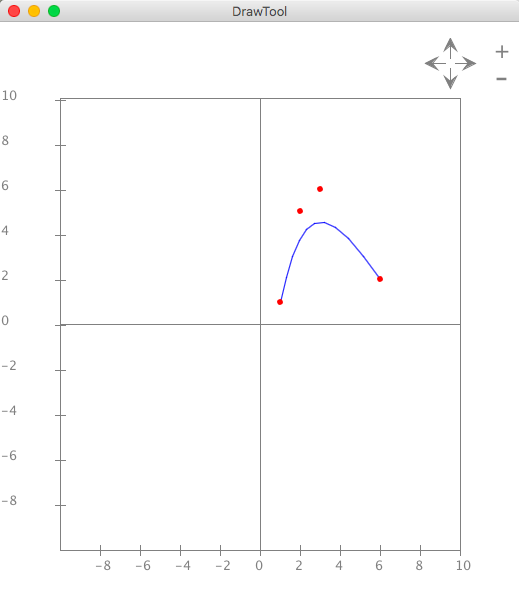
\includegraphics[scale=0.3]{exercise27}

%exercise 28
\item 4 control points: \\
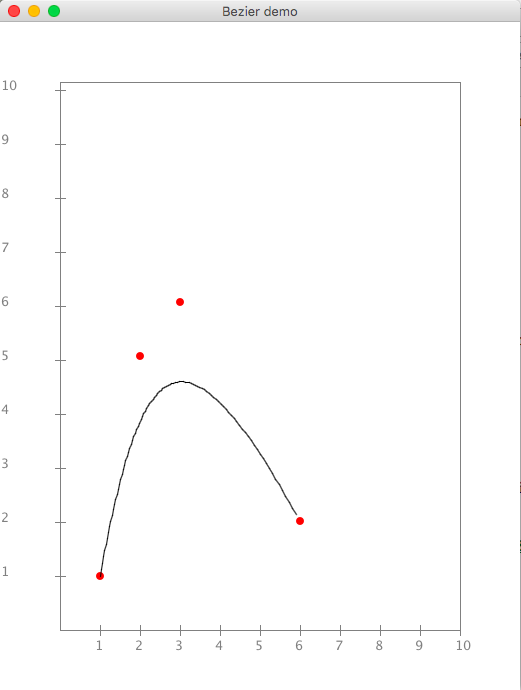
\includegraphics[scale=0.3]{exercise28_4}\\
10 control points:\\
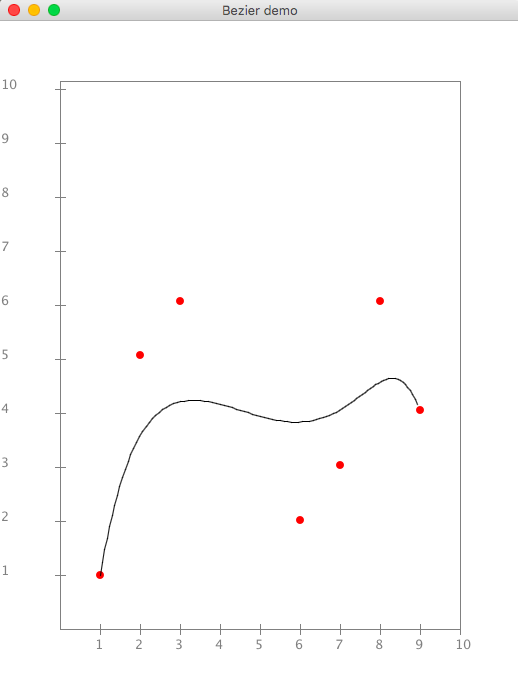
\includegraphics[scale=0.3]{exercise28}

%exercise 29
\item You don't get the surface, you get a line instead. A linear combination will give you a collection of points. If you want a surface, you need to start with surfaces. 
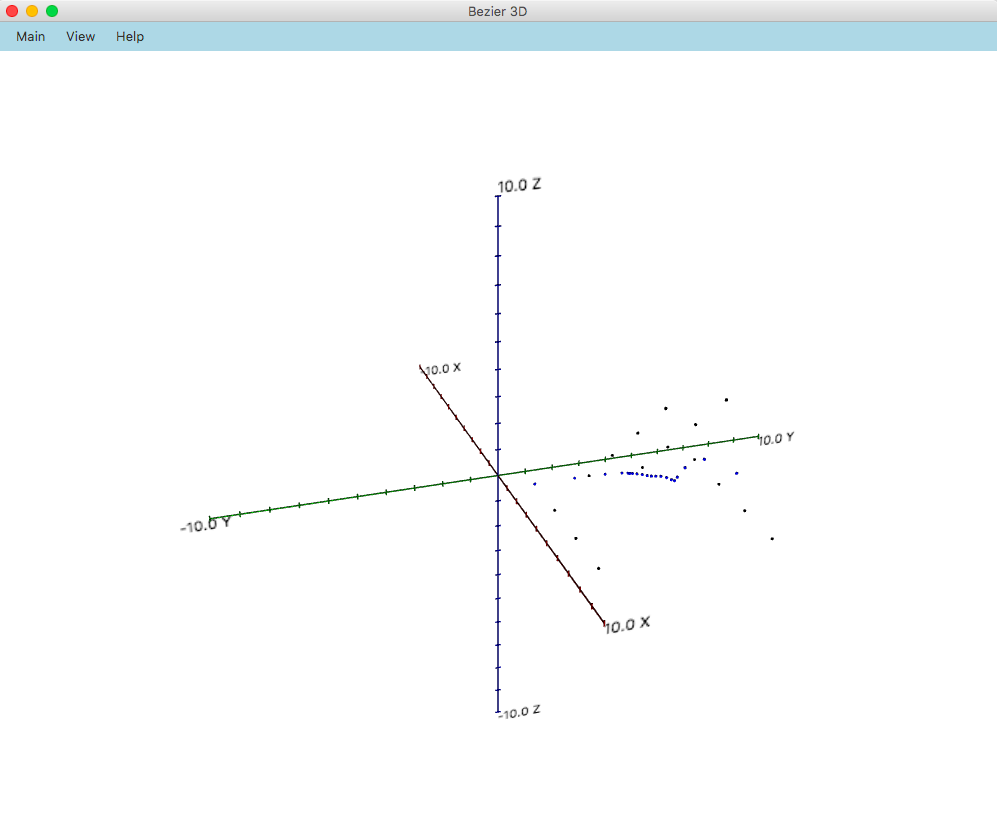
\includegraphics[scale=0.3]{exercise29}

%exercise 30
\item Bezier3D: \\
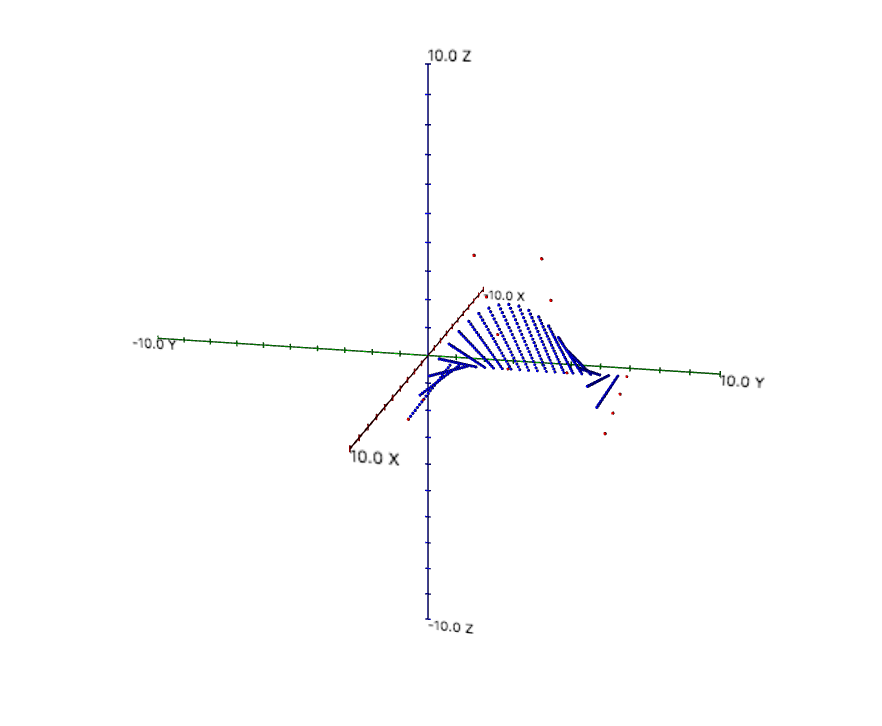
\includegraphics[scale=0.3]{exercise30}
%exercise 31
\item $n=3:$ \\
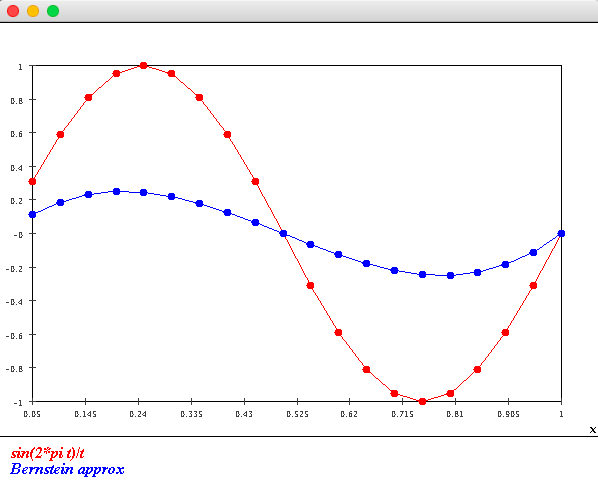
\includegraphics[scale=0.3]{bernstein_approx_3}\\
$n=10:$\\
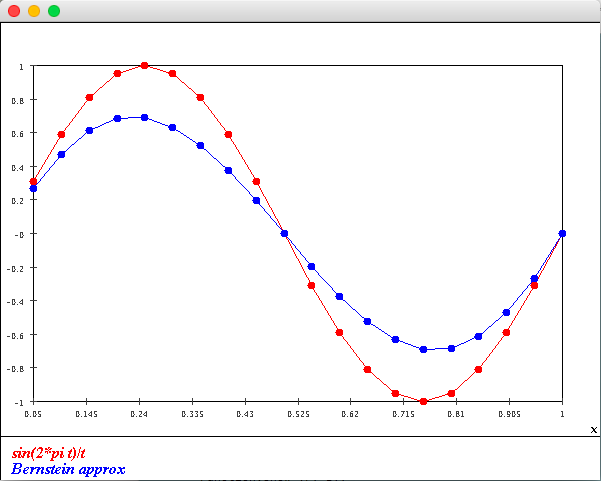
\includegraphics[scale=0.3]{bernstein_approx_10}
\end{enumerate}
\end{document}